\documentclass[12pt,a4paper]{article}

\usepackage[T1,T2A]{fontenc}
\usepackage[utf8]{inputenc}
\usepackage[russian]{babel}

%%%% Красная строка в русских текстах
\usepackage{indentfirst}

%%%% Настройка полей и отступов
\usepackage[a4paper,top=2cm,bottom=2cm,left=3cm,right=2cm,marginparwidth=1.75cm]{geometry}

%%%% Меняет стандартный формат нумерации секций
\usepackage{titlesec}
\titlelabel{\thetitle.\,\,}

%%%% Облегчают набор математических формул
\usepackage{amsmath}
\usepackage{amssymb}

%%%% Позволяют работать с графикой
\usepackage{graphicx}

%%%% Позволяет выделять текст цветом 
\usepackage{color}


\begin{document}

%%%%%%%%%%%%%%%%%%%%%%%%%%%
%%%%% ТИТУЛЬНЫЙ ЛИСТ %%%%%%
%%%%%%%%%%%%%%%%%%%%%%%%%%%
\begin{center} % включить выравнивание по центру
МИНИСТЕРСТВО ОБРАЗОВАНИЯ И НАУКИ РОССИЙСКОЙ \\
ФЕДЕРАЦИИ \\
Федеральное государственное автономное образовательное учреждение  \\
высшего образования\\ \textbf{<<Национальный исследовательский \\ Нижегородский государственный университет \\
им. Н.И. Лобачевского (ННГУ)>>}\\[1.5cm]%[4.5cm]
\textbf{Институт информационных технологий, математики и механики}\\[5.5cm]
%\textbf{Кафедра: Теории управления и динамики систем\\(ТУДС)}\\[0.8cm]
%Направление подготовки: \textbf{<<Математика и механика>>}\\
%направленность: \textbf{<<Дифференциальные уравнения, динамические системы и оптимальное управление>>}\\[2.2cm]

 \textbf{\large ОТЧЕТ} \\ % название работы, затем отступ 0,6см
 по \textbf{лабораторной} работе \\[0.6cm]
 
 на тему:\\
  \textbf{\large <<Исследование динамики системы с двумя параметрами>>}\\[6.5cm]
 % тема работы, затем отступ 3,7см
\begin{flushright}
 \begin{minipage}{0.52\textwidth} % начало маленькой врезки в половину ширины текста
 \begin{flushleft} % выровнять её содержимое по левому краю
  \textbf{Выполнил:} \\
 студент группы 3822Б1ПМ2 Махнёв Р.Д. \\
  \textbf{Проверил:}\\
 преподаватель каф. ТУДС Гринес Е.А.\\
 \end{flushleft} % конец выравнивания по левому краю
 \end{minipage} % конец врезки
\end{flushright}
 \vfill % заполнить всё доступное ниже пространство

  Нижний Новгород \\
 2024

 \thispagestyle{empty} % не нумеровать страницу

\end{center}

%%%%%%%%%%%%%%%%%%%%%%%%%%%%%%%%%%%%%
%%%%%%%% ОГЛАВЛЕНИЕ %%%%%%%%%%%%%%%%%
%%%%%%%%%%%%%%%%%%%%%%%%%%%%%%%%%%%%%
\renewcommand{\contentsname}{Содержание}
\newpage
\tableofcontents


%%%%%%%%%%%%%%%%%%%%%%%%%%%%%%%%%%%%%
%%%%%%%%% ОСНОВНАЯ ЧАСТЬ РАБОТЫ %%%%%
%%%%%%%%%%%%%%%%%%%%%%%%%%%%%%%%%%%%%
\newpage
\section{Анализ состояний равновесия системы}
Рассмотрим систему 
$$ 
\left \lbrace 
\begin{matrix}
\dot{x} = -x(b-x-y), \\
\dot{y} = (a-y)(2x+y).
\end{matrix} 
\right . .$$
Это нелинейная динамическая система, зависящая от параметров. Покажем, как построить для неё бифуркационную диаграмму.

% \subsection{Найти координаты всех состояний равновесия в зависимости от параметров}
Сначала найдём координаты всех присутствующих в ней состоянияй равновесия в зависимости от параметров.
Состояния равновесия находятся как решения системы уравнений 
$$ 
\left \lbrace 
\begin{matrix}
-x(b-x-y) =  0 \\
(a-y)(2x+y)  =  0
\end{matrix} 
\right . .$$
В результате получаем четыре состояния равновесия: $(0, 0)$, $(0, a)$, $( b-a , a)$ и 
$ ( -b, 2b) $.

%\subsection{Анализ матриц Якоби, поиск бифуркационных значений параметров}
Теперь найдём матрицу Якоби этой системы. Следуя стандартным обозначениям, примем $P(x, y) = -x(b-x-y)$ и $Q(x, y) = (a-y)(2x+y)$.
Вычислим частные производные:
$$ P'_x (x, y) = \frac{\partial}{\partial x}(-x(b-x-y)) = \frac{\partial (-x)}{\partial x} \cdot (b-x-y) - x \cdot \frac{\partial (b-x-y)}{\partial x} = 2x + y -b, $$
$$ P'_y (x, y) = \frac{\partial}{\partial y}(-x(b-x-y)) = \frac{\partial (-x)}{\partial y} \cdot (a-2x+3y) - x \cdot \frac{\partial(b-x-y)}{\partial y} = x, $$
$$ Q'_x (x, y) = \frac{\partial}{\partial x}((a-y)(2x+y)) = \frac{\partial (a-y)}{\partial x} \cdot (2x+y) + (a-y) \cdot \frac{\partial(2x+y)}{\partial x} = 2(a-y) = 2a-2y,$$
$$ Q'_y (x, y) = \frac{\partial}{\partial y}((a-y)(2x+y)) = \frac{\partial (a-y)}{\partial y} \cdot (2x+y) + (a-y) \cdot \frac{\partial(2x+y)}{\partial y} = a-2x-2y.$$

Подставим теперь координаты состояний равновесия и проанализируем собственные числа матриц Якоби. Матрица Якоби состояния равновесия равновесия $(0, 0)$ равна 
$$ \begin{pmatrix}
-b & 0 \\
2a & a 
\end{pmatrix} .$$
Матрица нижнетреугольная, а значит её собственные числа совпадают с её диагональными элементами:
$\lambda_1 = -b, \; \lambda_2 = a$. 
Собственные числа всегда вещественные, поэтому состояние равновесия может быть негрубым только когда одно из этих собственных чисел равно нулю. {\color{blue} Таким образом, бифуркационное множество для этого состояния равновесия -- $a = 0$ или $ b = 0$.} Опять же, так как мы явно знаем собственные числа матрицы Якоби, мы можем проанализировать тип состояния равновесия при любых значениях параметров: 
\begin{itemize}
	\item{$-b > 0, \; a > 0$ -- неустойчивый узел;}
	\item{$-b < 0, \; a < 0$ -- устойчивый узел;}
	\item{$-b > 0, \; a < 0$ или $-b < 0, \; a > 0$ -- седло.}
\end{itemize} 


Для состояния равновесия с координатами $(0, a)$ матрица Якоби равна
$$ \begin{pmatrix}
	a-b & 0 \\
	0 & -a 
\end{pmatrix} .$$

Матрица диагональная, а значит её собственные числа совпадают с её диагональными элементами:
$\lambda_1 = a-b, \; \lambda_2 = -a$. 
Собственные числа всегда вещественные, поэтому состояние равновесия может быть негрубым только когда одно из этих собственных чисел равно нулю. {\color{blue} Таким образом, бифуркационное множество для этого состояния равновесия -- $a = b$ или $ a = 0$.} 
Так как мы явно знаем собственные числа матрицы Якоби, мы можем проанализировать тип состояния равновесия при любых значениях параметров:  
\begin{itemize}
	\item{$a-b > 0, \; -a > 0$ -- неустойчивый узел;}
	\item{$a-b < 0, \; -a < 0$ -- устойчивый узел;}
	\item{$a-b > 0, \; -a < 0$ или $a-b < 0, \; -a > 0$ -- седло.}
\end{itemize}



Матрица Якоби, вычисленная в состоянии равновесия $\left ( b-a , a \right )$, равна   
$$ \begin{pmatrix}
	b-a & b-a \\
	0 & a-2b
\end{pmatrix} .$$
Матрица верхнетреугольная, а значит её собственные числа совпадают с её диагональными элементами:
$\lambda_1 = b-a, \; \lambda_2 = a-2b$. 
Собственные числа всегда вещественные, поэтому состояние равновесия может быть негрубым только когда одно из этих собственных чисел равно нулю. {\color{blue} Таким образом, бифуркационное множество для этого состояния равновесия -- $a = b$ или $ a = 2b$.} Поскольку здесь мы также явно знаем собственные числа матрицы Якоби, то мы можем проанализировать тип состояния равновесия при любых значениях параметров: 
\begin{itemize}
	\item{$b-a > 0, \; a-2b > 0$ -- неустойчивый узел;}
	\item{$b-a < 0, \; a-2b < 0$ -- устойчивый узел;}
	\item{$b-a > 0, \; a-2b < 0$ или $b-a < 0, \; a-2b > 0$ -- седло.}
\end{itemize}


Наконец, матрица Якоби в состоянии равновесия с координатами $ \left ( -b, 2b \right ) $  равна 
$$ \begin{pmatrix}
	-b & -b \\
	2a-4b &  a-2b
\end{pmatrix} .$$
Она не имеет какой-либо удобной структуры, поэтому для её исследования нужно исследовать её определитель и след:
$$ {\rm tr}\, J = a-3b $$
$$ {\rm det}\, J = 
-b \cdot (a-2b) + b \cdot (2a-4b) = 
b \cdot ( 2a-4b - (a-2b))  = b \cdot \left ( a-2b) \right. $$
Сначала проанализируем первое вырождение состояния равновесия, а именно -- наличие как минимум одного нулевого собственного число. 
Для этого определитель должен обратиться в ноль: 
$$ {\rm det}\, J = b \cdot \left ( a-2b) = 0\right.$$
Это уравнение имеет решения
$$
\left \lbrack 
\begin{matrix}
	b = 0 \\
	a = 2b
\end{matrix}
\right . .
$$
Проверим, имеет ли место второе вырождение 
$$ {\rm tr}\, J = 0, \; {\rm det}\, J > 0.$$
Для этого сначала решим уравнение ${\rm tr}\, J = 0$:
$${\rm tr}\, J = a-3b = 0,$$
откуда $a = 3b$.
Подставим теперь это в выражение для определителя.
Получим 
$$  b \cdot  ( a-2b) = b \cdot  ( 3b-2b) = b \cdot  b = b^2 \geq 0.$$
Таким образом, при $a = 3b, b \neq 0$ происходит второе вырождение, при котором у матрицы Якоби состояния равновесия появляется пара чисто мнимых собственных
чисел.
{\color{blue} Результирующее бифуркационное множество есть $b \cdot ( a-2b)=0$ или $a = 3b $ (при $b \ne 0 $).} С помощью следа и определителя мы можем определить, при каких значениях параметров данное состояние равновесия имеет определённый тип:
\begin{itemize}
	\item{$b \cdot ( a-2b) < 0$ -- седло (${\rm det}\, J < 0$); }
	\item{$b \cdot ( a-2b) > 0, \; a-3b > 0$ -- неустойчивый узел/фокус (${\rm det}\, J > 0, \; {\rm tr}\, J > 0$);}
	\item{$b \cdot ( a-2b) > 0, \; a-3b < 0$ -- устойчивый узел/фокус (${\rm det}\, J > 0, \; {\rm tr}\, J < 0$).}
\end{itemize} 


\subsection{Общая бифуркационная диаграмма для всех состояний равновесия}
Выпишем бифуркационное множество для всех состояний равновесия: 
\begin{itemize}
\item{$a = 0$ или $ b = 0$ для $(0, 0)$;}
\item{$a = b$ или $ a = 0$ для $(0, a)$;}
\item{$a = b$ или $ a = 2b$ для $\left (b-a , a \right )$;}
\item{$b = 0$ или $(a-2b)=0$ или $a = 3b $ (при $b \ne 0 $)  для $ \left ( -b, 2b  \right ) $.}
\end{itemize}
Воспользуемся GeoGebra для построения бифуркационного множества (по оси $x$ параметр $a$, а по оси $y$ -- параметр $b$).
\begin{figure}[!thb]
\includegraphics[height=8cm]{Bifdiag.png}
\centering
\caption{\label{fig:bifdiag2} Бифуркационные границы данной системы.}
\end{figure}
Определить тип каждого состояния равновесия можно двумя способами.
Во-первых, с помощью GeoGebra можно построить любое сочетание неравенств, которые определяют тип состояний равновесия.
Во-вторых, это можно сделать, взяв какие-нибудь конкретные значения параметров и проверив, какому из неравенств удовлетворяют значения параметров. 
Возьмем, например, $a^\ast = -4,\; b^\ast = 4$. 
Пересмотрим наши записи для каждого состояния равновесия: 
\begin{itemize}
\item{так как $-b^\ast < 0$ и $a^\ast < 0$, то $(0, 0)$ -- устойчивый узел;}
\item{так как $a^\ast -b^\ast < 0, \; -a^\ast > 0$, то $(0, a^\ast)$ -- седло; }
\item{так как $b^\ast-a^\ast > 0, \; a^\ast - 2b^\ast < 0$ , то $\left ( b^\ast-a^\ast , a^\ast \right )$ -- седло;}
\item{так как $b^\ast(a^\ast - 2 b^\ast) < 0$, то $  ( -b^\ast, 2b^\ast ) $ -- седло.}
\end{itemize}
\subsection{Поиск инвариантных прямых}
\newpage

\section{Фазовые портреты системы}
При построении фазовых портретов системы будем пользоваться конкретными значениями параметров из выбранной области. Это позволит узнать тип каждого состояния равновесия: для этого нужно проверить, какому из неравенств удовлетворяют значения параметров.

\subsection{Область 1}
Выберем точку на бифуркационной диаграмме $(a^\ast = 0$, $b^\ast = 15)$. Она соответствует следующим значениям параметров:  $a^\ast = 0$, $b^\ast = 15$. При этих параметрах система будет иметь следующий вид: 

$$
\left \lbrace 
\begin{matrix} 
	\dot{x} = -x \cdot (-x - y + 15), \\
	\dot{y} = -y \cdot (2 \cdot x + y). \
\end{matrix} 
\right . .$$

Состояния равновесия данной системы:  $(0, 0)$, $(-15, 30)$, $(15, 0)$. Определим тип каждого состояния равновесия, проверив, какому из неравенств удовлетворяют взятые значения параметров.  Пересмотрим наши записи для каждого состояния равновесия: 
\begin{itemize}
	\item{ так как $-b^\ast  < 0 $ и $a^\ast = 0 $ то $(0, 0)$ -- седлоузел. Найдём ведущее направление данного узла. Якобиан в состоянии равновесия $(0, 0)$ выглядит следующим образом:
		
		$$\begin{pmatrix}-15 & 0\\0 & 0\end{pmatrix}. $$Её собственные числа это $\lambda_1=-15$, которому соотвествует вектор $\Vec{V_1}=$ $\left[\begin{matrix}1\\0\end{matrix}\right]$ и $\lambda_2=0$, которому соотвествует вектор $\Vec{V_2}=$$\left[\begin{matrix}0\\1\end{matrix}\right]$.Так как $\lambda_2=0$ ближайшее к $0$ собственное число, то при подходе к состоянию равновесия траектории будут стремиться к направлению, задаваемому вектором $\Vec{V_2}=$ $\left[\begin{matrix}0\\1\end{matrix}\right]$;}

	\item{ так как ${\lambda_{1}} = - \frac{15 \sqrt{17}}{2} - \frac{45}{2}$$  < 0 $ и ${\lambda_{2}} = - \frac{45}{2} + \frac{15 \sqrt{17}}{2}$$ > 0 $ то $(-15, 30)$ -- седло;}
	\item{ так как $-a^\ast + b^\ast > 0 $ и $a^\ast - 2*b^\ast  < 0 $ то $(15, 0)$ -- седло.}
\end{itemize} 
В данном случае произошла транскритическая бифуркация. Выпишем всё, что потребуется при построении фазового портрета:
Уравнения нульклин имеют следующий вид: 

$$x=0$$
$$y=15 - x$$
$$x=- \frac{y}{2}$$
$$y=0$$


Уравнения инвариантных прямых имеют следующий вид: 
$$y = 0$$
$$x = 0$$



Построим фазовый портрет (Рис. \ref{fig:phportr01}).

\begin{figure}[h]
	\includegraphics[width=\textwidth]{phptr/(0,15).jpg}
	\centering
	\caption{\label{fig:phportr01} Фазовый портрет системы с параметрами $a^\ast = 0$, $b^\ast = 15$.}
\end{figure}



\subsection{Область 2}

Выберем точку на бифуркационной диаграмме $(a^\ast = 0$, $b^\ast = 0)$. Она соответствует следующим значениям параметров:  $a^\ast = 0$, $b^\ast = 0$. При этих параметрах система будет иметь следующий вид: 

$$
\left \lbrace 
\begin{matrix} 
	\dot{x} = -x \cdot (-x - y), \\
	\dot{y} = -y \cdot (2 \cdot x + y). \
\end{matrix} 
\right . .$$

Единственное состояние равновесия данной системы: $(0, 0)$.

Выпишем всё, что потребуется при построении фазового портрета:

Уравнения нульклин имеют следующий вид: 

$$x=0$$
$$y=- x$$
$$x=- \frac{y}{2}$$
$$y=0$$


Уравнения инвариантных прямых имеют следующий вид: 
$$y = - \frac{3 x}{2}$$
$$y = 0$$
$$x = - \frac{2 y}{3}$$
$$x = 0$$



Построим фазовый портрет (Рис. \ref{fig:phportr02}).
\newpage
\begin{figure}[h]
	\includegraphics[width=\textwidth]{phptr/(0, 0).jpg}
	\centering
	\caption{\label{fig:phportr02} Фазовый портрет системы с параметрами $(a^\ast = 0$, $b^\ast = 0)$.}
\end{figure}

\subsection{Область 3}

Выберем точку на бифуркационной диаграмме $(0, -9)$. Она соответствует следующим значениям параметров:  $a^\ast = 0$, $b^\ast = -9$. При этих параметрах система будет иметь следующий вид: 

$$
\left \lbrace 
\begin{matrix} 
	\dot{x} = -x \cdot (-x - y - 9), \\
	\dot{y} = -y \cdot (2 \cdot x + y). \
\end{matrix} 
\right . .$$

Состояния равновесия данной системы: $(0, 0)$, $(9, -18)$, $(-9, 0)$. Определим тип каждого состояния равновесия, проверив, какому из неравенств удовлетворяют взятые значения параметров.  Пересмотрим наши записи для каждого состояния равновесия: 
\begin{itemize}
	\item{ так как $-b^\ast > 0 $ и $a^\ast = 0 $ то $(0, 0)$ -- седлоузел. Найдём ведущее направление данного узла. Якобиан в состоянии равновесия $(0, 0)$ выглядит следующим образом:
		
		$$\begin{pmatrix}9 & 0\\0 & 0\end{pmatrix}. $$Её собственные числа это $\lambda_1=0$, которому соотвествует вектор $\Vec{V_1}=$ $\left[\begin{matrix}0\\1\end{matrix}\right]$ и $\lambda_2=9$, которому соотвествует вектор $\Vec{V_2}=$$\left[\begin{matrix}1\\0\end{matrix}\right]$.Так как $\lambda_1=0$ ближайшее к $0$ собственное число, то при подходе к состоянию равновесия траектории будут стремиться к направлению, задаваемому вектором $\Vec{V_1}=$ $\left[\begin{matrix}0\\1\end{matrix}\right]$;}
	\item{ так как ${\lambda_{1}} = \frac{27}{2} - \frac{9 \sqrt{17}}{2}$$  < 0 $ и ${\lambda_{2}} = \frac{27}{2} + \frac{9 \sqrt{17}}{2}$$ > 0 $ то $(9, -18)$ -- седло;}
	\item{ так как $-a^\ast + b^\ast  < 0 $ и $a^\ast - 2*b^\ast > 0 $ то $(-9, 0)$ -- седло.}
\end{itemize} 

В данном случае произошла транскритическая бифуркация. Выпишем всё, что потребуется при построении фазового портрета:

Уравнения нульклин имеют следующий вид: 

$$x=0$$
$$y=- x - 9$$
$$x=- \frac{y}{2}$$
$$y=0$$


Уравнения инвариантных прямых имеют следующий вид: 
$$y = 0$$
$$x = 0$$

Построим фазовый портрет (Рис. \ref{fig:phportr03}).
\begin{figure}[h]
	\includegraphics[width=\textwidth]{phptr/(0,-9) транскритическая).jpg}
	\centering
	\caption{\label{fig:phportr03} Фазовый портрет системы с параметрами $a^\ast = 0$, $b^\ast = -9$.}
\end{figure}

\newpage
RunGenerator
\newpage


\subsection{Область 4}

Выберем точку на бифуркационной диаграмме $(8, 8)$. Она соответствует следующим значениям параметров:  $a^\ast = 8$, $b^\ast = 8$. При этих параметрах система будет иметь следующий вид: 

$$
\left \lbrace 
\begin{matrix} 
	\dot{x} = -x \cdot (-x - y + 8), \\
	\dot{y} = (8 - y) \cdot (2 \cdot x + y). \
\end{matrix} 
\right . .$$

Состояния равновесия данной системы: $(0, 0)$, $(0, 8)$, $(-8, 16)$, $(0, 8)$. Определим тип каждого состояния равновесия, проверив, какому из неравенств удовлетворяют взятые значения параметров.  Пересмотрим наши записи для каждого состояния равновесия: 
\begin{itemize}
	\item{ так как $-b^\ast  < 0 $ и $a^\ast > 0 $ то $(0, 0)$ -- седло;}
	\item{ так как $a^\ast - b^\ast = 0 $ и $-a^\ast  < 0 $ то $(0, 8)$ -- седлоузел. Найдём ведущее направление данного узла. Якобиан в состоянии равновесия $(0, a)$ выглядит следующим образом:
		
		$$\begin{pmatrix}0 & 0\\0 & -8\end{pmatrix}. $$Её собственные числа это $\lambda_1=-8$, которому соотвествует вектор $\Vec{V_1}=$ $\left[\begin{matrix}0\\1\end{matrix}\right]$ и $\lambda_2=0$, которому соотвествует вектор $\Vec{V_2}=$$\left[\begin{matrix}1\\0\end{matrix}\right]$.Так как $\lambda_2=0$ ближайшее к $0$ собственное число, то при подходе к состоянию равновесия траектории будут стремиться к направлению, задаваемому вектором $\Vec{V_2}=$ $\left[\begin{matrix}1\\0\end{matrix}\right]$;}
	\item{ так как ${\lambda_{1}} = - 8 \sqrt{2} - 8$$  < 0 $ и ${\lambda_{2}} = -8 + 8 \sqrt{2}$$ > 0 $ то $(-8, 16)$ -- седло;}
	\item{ так как $-a^\ast + b^\ast = 0 $ и $a^\ast - 2*b^\ast  < 0 $ то $(0, 8)$ -- седлоузел. Найдём ведущее направление данного узла. Якобиан в состоянии равновесия $(-a + b, a)$ выглядит следующим образом:
		
		$$\begin{pmatrix}0 & 0\\0 & -8\end{pmatrix}. $$Её собственные числа это $\lambda_1=-8$, которому соотвествует вектор $\Vec{V_1}=$ $\left[\begin{matrix}0\\1\end{matrix}\right]$ и $\lambda_2=0$, которому соотвествует вектор $\Vec{V_2}=$$\left[\begin{matrix}1\\0\end{matrix}\right]$.Так как $\lambda_2=0$ ближайшее к $0$ собственное число, то при подходе к состоянию равновесия траектории будут стремиться к направлению, задаваемому вектором $\Vec{V_2}=$ $\left[\begin{matrix}1\\0\end{matrix}\right]$.}
\end{itemize} 

Выпишем всё, что потребуется при построении фазового портрета:

Уравнения нульклин имеют следующий вид: 

$$x=0$$
$$y=8 - x$$
$$x=- \frac{y}{2}$$
$$y=8$$


Уравнения инвариантных прямых имеют следующий вид: 
$$y = 8$$
$$x = 0$$
Построим фазовый портрет (Рис. \ref{fig:phportr4}).

\begin{figure}[h]
	
	\includegraphics[width=\textwidth]{phptr/(8, 4) транскритическая.jpg}
	\centering
	\caption{\label{fig:phportr4} Фазовый портрет системы с параметрами $a^\ast = 8$, $b^\ast = 8$.}
	
\end{figure}

\subsection{Область 5}

Выберем точку на бифуркационной диаграмме $(2, 2)$. Она соответствует следующим значениям параметров:  $a^\ast = 2$, $b^\ast = 2$. При этих параметрах система будет иметь следующий вид: 

$$
\left \lbrace 
\begin{matrix} 
	\dot{x} = -x \cdot (-x - y + 2), \\
	\dot{y} = (2 - y) \cdot (2 \cdot x + y). \
\end{matrix} 
\right . .$$

Состояния равновесия данной системы: $(0, 0)$, $(0, 2)$, $(-2, 4)$, $(0, 2)$. Определим тип каждого состояния равновесия, проверив, какому из неравенств удовлетворяют взятые значения параметров.  Пересмотрим наши записи для каждого состояния равновесия: 
\begin{itemize}
	\item{ так как $-b^\ast  < 0 $ и $a^\ast > 0 $ то $(0, 0)$ -- седло;}
	\item{ так как $a^\ast - b^\ast = 0 $ и $-a^\ast  < 0 $ то $(0, 2)$ -- седлоузел. Найдём ведущее направление данного узла. Якобиан в состоянии равновесия $(0, a)$ выглядит следующим образом:
		
		$$\begin{pmatrix}0 & 0\\0 & -2\end{pmatrix}. $$Её собственные числа это $\lambda_1=-2$, которому соотвествует вектор $\Vec{V_1}=$ $\left[\begin{matrix}0\\1\end{matrix}\right]$ и $\lambda_2=0$, которому соотвествует вектор $\Vec{V_2}=$$\left[\begin{matrix}1\\0\end{matrix}\right]$.Так как $\lambda_2=0$ ближайшее к $0$ собственное число, то при подходе к состоянию равновесия траектории будут стремиться к направлению, задаваемому вектором $\Vec{V_2}=$ $\left[\begin{matrix}1\\0\end{matrix}\right]$;}
	\item{ так как ${\lambda_{1}} = - 2 \sqrt{2} - 2$$  < 0 $ и ${\lambda_{2}} = -2 + 2 \sqrt{2}$$ > 0 $ то $(-2, 4)$ -- седло;}
	\item{ так как $-a^\ast + b^\ast = 0 $ и $a^\ast - 2*b^\ast  < 0 $ то $(0, 2)$ -- седлоузел. Найдём ведущее направление данного узла. Якобиан в состоянии равновесия $(-a + b, a)$ выглядит следующим образом:
		
		$$\begin{pmatrix}0 & 0\\0 & -2\end{pmatrix}. $$Её собственные числа это $\lambda_1=-2$, которому соотвествует вектор $\Vec{V_1}=$ $\left[\begin{matrix}0\\1\end{matrix}\right]$ и $\lambda_2=0$, которому соотвествует вектор $\Vec{V_2}=$$\left[\begin{matrix}1\\0\end{matrix}\right]$.Так как $\lambda_2=0$ ближайшее к $0$ собственное число, то при подходе к состоянию равновесия траектории будут стремиться к направлению, задаваемому вектором $\Vec{V_2}=$ $\left[\begin{matrix}1\\0\end{matrix}\right]$.}
\end{itemize} 

Выпишем всё, что потребуется при построении фазового портрета:

Уравнения нульклин имеют следующий вид: 

$$x=0$$
$$y=2 - x$$
$$x=- \frac{y}{2}$$
$$y=2$$


Уравнения инвариантных прямых имеют следующий вид: 
$$y = 2$$
$$x = 0$$
Построим фазовый портрет (Рис. \ref{fig:phportr5}).

\begin{figure}[h]
	
	\includegraphics[width=\textwidth]{phptr/(2,2).jpg}
	\centering
	\caption{\label{fig:phportr5} Фазовый портрет системы с параметрами $a^\ast = 2$, $b^\ast = 2$.}
	
\end{figure}

\subsection{Область 6}

Выберем точку на бифуркационной диаграмме $(-2, -2)$. Она соответствует следующим значениям параметров:  $a^\ast = -2$, $b^\ast = -2$. При этих параметрах система будет иметь следующий вид: 

$$
\left \lbrace 
\begin{matrix} 
	\dot{x} = -x \cdot (-x - y - 2), \\
	\dot{y} = (2 \cdot x + y) \cdot (-y - 2). \
\end{matrix} 
\right . .$$

Состояния равновесия данной системы: $(0, 0)$, $(0, -2)$, $(2, -4)$, $(0, -2)$. Определим тип каждого состояния равновесия, проверив, какому из неравенств удовлетворяют взятые значения параметров.  Пересмотрим наши записи для каждого состояния равновесия: 
\begin{itemize}
	\item{ так как $-b^\ast > 0 $ и $a^\ast  < 0 $ то $(0, 0)$ -- седло;}
	\item{ так как $a^\ast - b^\ast = 0 $ и $-a^\ast > 0 $ то $(0, -2)$ -- седлоузел. Найдём ведущее направление данного узла. Якобиан в состоянии равновесия $(0, a)$ выглядит следующим образом:
		
		$$\begin{pmatrix}0 & 0\\0 & 2\end{pmatrix}. $$Её собственные числа это $\lambda_1=0$, которому соотвествует вектор $\Vec{V_1}=$ $\left[\begin{matrix}1\\0\end{matrix}\right]$ и $\lambda_2=2$, которому соотвествует вектор $\Vec{V_2}=$$\left[\begin{matrix}0\\1\end{matrix}\right]$.Так как $\lambda_1=0$ ближайшее к $0$ собственное число, то при подходе к состоянию равновесия траектории будут стремиться к направлению, задаваемому вектором $\Vec{V_1}=$ $\left[\begin{matrix}1\\0\end{matrix}\right]$;}
	\item{ так как ${\lambda_{1}} = 2 - 2 \sqrt{2}$$  < 0 $ и ${\lambda_{2}} = 2 + 2 \sqrt{2}$$ > 0 $ то $(2, -4)$ -- седло;}
	\item{ так как $-a^\ast + b^\ast = 0 $ и $a^\ast - 2*b^\ast > 0 $ то $(0, -2)$ -- седлоузел. Найдём ведущее направление данного узла. Якобиан в состоянии равновесия $(-a + b, a)$ выглядит следующим образом:
		
		$$\begin{pmatrix}0 & 0\\0 & 2\end{pmatrix}. $$Её собственные числа это $\lambda_1=0$, которому соотвествует вектор $\Vec{V_1}=$ $\left[\begin{matrix}1\\0\end{matrix}\right]$ и $\lambda_2=2$, которому соотвествует вектор $\Vec{V_2}=$$\left[\begin{matrix}0\\1\end{matrix}\right]$.Так как $\lambda_1=0$ ближайшее к $0$ собственное число, то при подходе к состоянию равновесия траектории будут стремиться к направлению, задаваемому вектором $\Vec{V_1}=$ $\left[\begin{matrix}1\\0\end{matrix}\right]$.}
\end{itemize} 

Выпишем всё, что потребуется при построении фазового портрета:

Уравнения нульклин имеют следующий вид: 

$$x=0$$
$$y=- x - 2$$
$$x=- \frac{y}{2}$$
$$y=-2$$


Уравнения инвариантных прямых имеют следующий вид: 
$$y = -2$$
$$x = 0$$
Построим фазовый портрет (Рис. \ref{fig:phportr6}).

\begin{figure}[h]
	
	\includegraphics[width=\textwidth]{phptr/(-2, -2) транскритическая.jpg}
	\centering
	\caption{\label{fig:phportr6} Фазовый портрет системы с параметрами $a^\ast = -2$, $b^\ast = -2$.}
	
\end{figure}

\subsection{Область 7}

Выберем точку на бифуркационной диаграмме $(-2, -2)$. Она соответствует следующим значениям параметров:  $a^\ast = -2$, $b^\ast = -2$. При этих параметрах система будет иметь следующий вид: 

$$
\left \lbrace 
\begin{matrix} 
	\dot{x} = -x \cdot (-x - y - 2), \\
	\dot{y} = (2 \cdot x + y) \cdot (-y - 2). \
\end{matrix} 
\right . .$$

Состояния равновесия данной системы: $(0, 0)$, $(0, -2)$, $(2, -4)$, $(0, -2)$. Определим тип каждого состояния равновесия, проверив, какому из неравенств удовлетворяют взятые значения параметров.  Пересмотрим наши записи для каждого состояния равновесия: 
\begin{itemize}
	\item{ так как $-b^\ast > 0 $ и $a^\ast  < 0 $ то $(0, 0)$ -- седло;}
	\item{ так как $a^\ast - b^\ast = 0 $ и $-a^\ast > 0 $ то $(0, -2)$ -- седлоузел. Найдём ведущее направление данного узла. Якобиан в состоянии равновесия $(0, a)$ выглядит следующим образом:
		
		$$\begin{pmatrix}0 & 0\\0 & 2\end{pmatrix}. $$Её собственные числа это $\lambda_1=0$, которому соотвествует вектор $\Vec{V_1}=$ $\left[\begin{matrix}1\\0\end{matrix}\right]$ и $\lambda_2=2$, которому соотвествует вектор $\Vec{V_2}=$$\left[\begin{matrix}0\\1\end{matrix}\right]$.Так как $\lambda_1=0$ ближайшее к $0$ собственное число, то при подходе к состоянию равновесия траектории будут стремиться к направлению, задаваемому вектором $\Vec{V_1}=$ $\left[\begin{matrix}1\\0\end{matrix}\right]$;}
	\item{ так как ${\lambda_{1}} = 2 - 2 \sqrt{2}$$  < 0 $ и ${\lambda_{2}} = 2 + 2 \sqrt{2}$$ > 0 $ то $(2, -4)$ -- седло;}
	\item{ так как $-a^\ast + b^\ast = 0 $ и $a^\ast - 2*b^\ast > 0 $ то $(0, -2)$ -- седлоузел. Найдём ведущее направление данного узла. Якобиан в состоянии равновесия $(-a + b, a)$ выглядит следующим образом:
		
		$$\begin{pmatrix}0 & 0\\0 & 2\end{pmatrix}. $$Её собственные числа это $\lambda_1=0$, которому соотвествует вектор $\Vec{V_1}=$ $\left[\begin{matrix}1\\0\end{matrix}\right]$ и $\lambda_2=2$, которому соотвествует вектор $\Vec{V_2}=$$\left[\begin{matrix}0\\1\end{matrix}\right]$.Так как $\lambda_1=0$ ближайшее к $0$ собственное число, то при подходе к состоянию равновесия траектории будут стремиться к направлению, задаваемому вектором $\Vec{V_1}=$ $\left[\begin{matrix}1\\0\end{matrix}\right]$.}
\end{itemize} 

Выпишем всё, что потребуется при построении фазового портрета:

Уравнения нульклин имеют следующий вид: 

$$x=0$$
$$y=- x - 2$$
$$x=- \frac{y}{2}$$
$$y=-2$$


Уравнения инвариантных прямых имеют следующий вид: 
$$y = -2$$
$$x = 0$$
Построим фазовый портрет (Рис. \ref{fig:phportr7}).

\begin{figure}[h]
	
	\includegraphics[width=\textwidth]{phptr/(-20, -7).jpeg}
	\centering
	\caption{\label{fig:phportr7} Фазовый портрет системы с параметрами $a^\ast = -2$, $b^\ast = -2$.}
	
\end{figure}

\subsection{Область 8}

Выберем точку на бифуркационной диаграмме $(-3, -3)$. Она соответствует следующим значениям параметров:  $a^\ast = -3$, $b^\ast = -3$. При этих параметрах система будет иметь следующий вид: 

$$
\left \lbrace 
\begin{matrix} 
	\dot{x} = -x \cdot (-x - y - 3), \\
	\dot{y} = (2 \cdot x + y) \cdot (-y - 3). \
\end{matrix} 
\right . .$$

Состояния равновесия данной системы: $(0, 0)$, $(0, -3)$, $(3, -6)$, $(0, -3)$. Определим тип каждого состояния равновесия, проверив, какому из неравенств удовлетворяют взятые значения параметров.  Пересмотрим наши записи для каждого состояния равновесия: 
\begin{itemize}
	\item{ так как $-b^\ast > 0 $ и $a^\ast  < 0 $ то $(0, 0)$ -- седло;}
	\item{ так как $a^\ast - b^\ast = 0 $ и $-a^\ast > 0 $ то $(0, -3)$ -- седлоузел. Найдём ведущее направление данного узла. Якобиан в состоянии равновесия $(0, a)$ выглядит следующим образом:
		
		$$\begin{pmatrix}0 & 0\\0 & 3\end{pmatrix}. $$Её собственные числа это $\lambda_1=0$, которому соотвествует вектор $\Vec{V_1}=$ $\left[\begin{matrix}1\\0\end{matrix}\right]$ и $\lambda_2=3$, которому соотвествует вектор $\Vec{V_2}=$$\left[\begin{matrix}0\\1\end{matrix}\right]$.Так как $\lambda_1=0$ ближайшее к $0$ собственное число, то при подходе к состоянию равновесия траектории будут стремиться к направлению, задаваемому вектором $\Vec{V_1}=$ $\left[\begin{matrix}1\\0\end{matrix}\right]$;}
	\item{ так как ${\lambda_{1}} = 3 - 3 \sqrt{2}$$  < 0 $ и ${\lambda_{2}} = 3 + 3 \sqrt{2}$$ > 0 $ то $(3, -6)$ -- седло;}
	\item{ так как $-a^\ast + b^\ast = 0 $ и $a^\ast - 2*b^\ast > 0 $ то $(0, -3)$ -- седлоузел. Найдём ведущее направление данного узла. Якобиан в состоянии равновесия $(-a + b, a)$ выглядит следующим образом:
		
		$$\begin{pmatrix}0 & 0\\0 & 3\end{pmatrix}. $$Её собственные числа это $\lambda_1=0$, которому соотвествует вектор $\Vec{V_1}=$ $\left[\begin{matrix}1\\0\end{matrix}\right]$ и $\lambda_2=3$, которому соотвествует вектор $\Vec{V_2}=$$\left[\begin{matrix}0\\1\end{matrix}\right]$.Так как $\lambda_1=0$ ближайшее к $0$ собственное число, то при подходе к состоянию равновесия траектории будут стремиться к направлению, задаваемому вектором $\Vec{V_1}=$ $\left[\begin{matrix}1\\0\end{matrix}\right]$.}
\end{itemize} 

Выпишем всё, что потребуется при построении фазового портрета:

Уравнения нульклин имеют следующий вид: 

$$x=0$$
$$y=- x - 3$$
$$x=- \frac{y}{2}$$
$$y=-3$$


Уравнения инвариантных прямых имеют следующий вид: 
$$y = -3$$
$$x = 0$$
Построим фазовый портрет (Рис. \ref{fig:phportr8}).

\begin{figure}[h]
	
	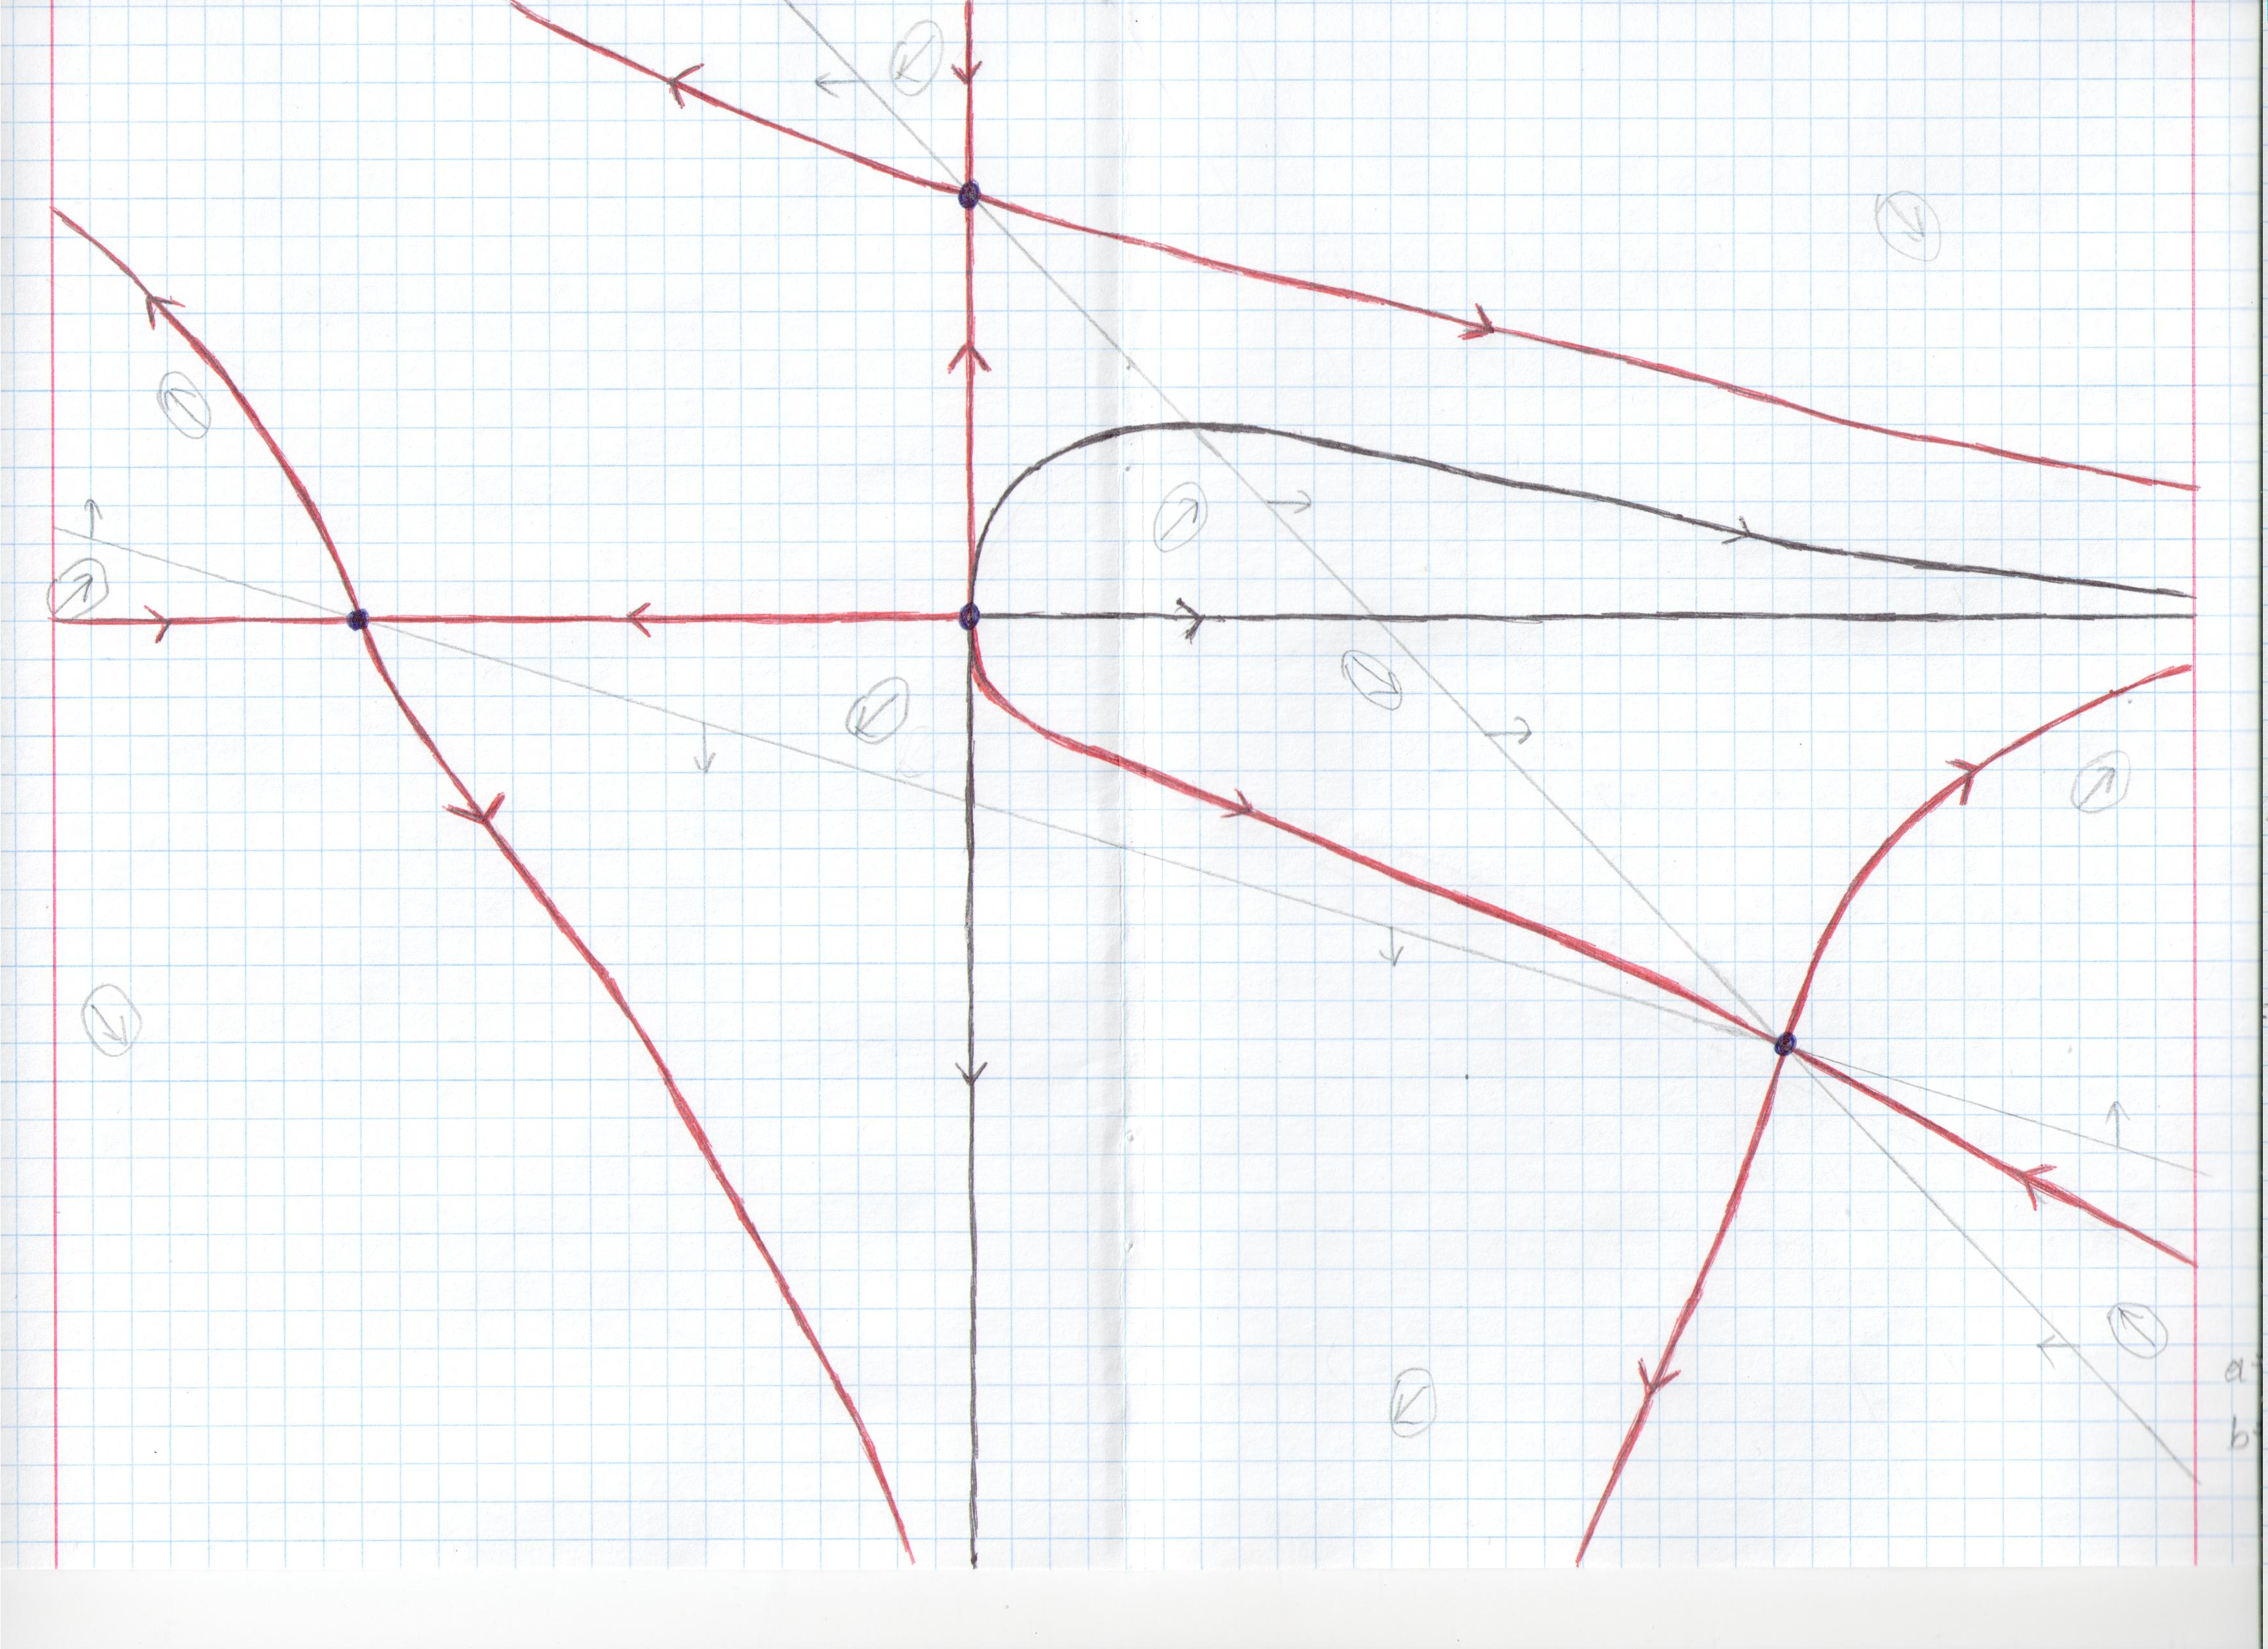
\includegraphics[width=\textwidth]{phptr/(-3,-9).jpg}
	\centering
	\caption{\label{fig:phportr8} Фазовый портрет системы с параметрами $a^\ast = -3$, $b^\ast = -3$.}
	
\end{figure}

\subsection{Область 9}

Выберем точку на бифуркационной диаграмме $(-6, -6)$. Она соответствует следующим значениям параметров:  $a^\ast = -6$, $b^\ast = -6$. При этих параметрах система будет иметь следующий вид: 

$$
\left \lbrace 
\begin{matrix} 
	\dot{x} = -x \cdot (-x - y - 6), \\
	\dot{y} = (2 \cdot x + y) \cdot (-y - 6). \
\end{matrix} 
\right . .$$

Состояния равновесия данной системы: $(0, 0)$, $(0, -6)$, $(6, -12)$, $(0, -6)$. Определим тип каждого состояния равновесия, проверив, какому из неравенств удовлетворяют взятые значения параметров.  Пересмотрим наши записи для каждого состояния равновесия: 
\begin{itemize}
	\item{ так как $-b^\ast > 0 $ и $a^\ast  < 0 $ то $(0, 0)$ -- седло;}
	\item{ так как $a^\ast - b^\ast = 0 $ и $-a^\ast > 0 $ то $(0, -6)$ -- седлоузел. Найдём ведущее направление данного узла. Якобиан в состоянии равновесия $(0, a)$ выглядит следующим образом:
		
		$$\begin{pmatrix}0 & 0\\0 & 6\end{pmatrix}. $$Её собственные числа это $\lambda_1=0$, которому соотвествует вектор $\Vec{V_1}=$ $\left[\begin{matrix}1\\0\end{matrix}\right]$ и $\lambda_2=6$, которому соотвествует вектор $\Vec{V_2}=$$\left[\begin{matrix}0\\1\end{matrix}\right]$.Так как $\lambda_1=0$ ближайшее к $0$ собственное число, то при подходе к состоянию равновесия траектории будут стремиться к направлению, задаваемому вектором $\Vec{V_1}=$ $\left[\begin{matrix}1\\0\end{matrix}\right]$;}
	\item{ так как ${\lambda_{1}} = 6 - 6 \sqrt{2}$$  < 0 $ и ${\lambda_{2}} = 6 + 6 \sqrt{2}$$ > 0 $ то $(6, -12)$ -- седло;}
	\item{ так как $-a^\ast + b^\ast = 0 $ и $a^\ast - 2*b^\ast > 0 $ то $(0, -6)$ -- седлоузел. Найдём ведущее направление данного узла. Якобиан в состоянии равновесия $(-a + b, a)$ выглядит следующим образом:
		
		$$\begin{pmatrix}0 & 0\\0 & 6\end{pmatrix}. $$Её собственные числа это $\lambda_1=0$, которому соотвествует вектор $\Vec{V_1}=$ $\left[\begin{matrix}1\\0\end{matrix}\right]$ и $\lambda_2=6$, которому соотвествует вектор $\Vec{V_2}=$$\left[\begin{matrix}0\\1\end{matrix}\right]$.Так как $\lambda_1=0$ ближайшее к $0$ собственное число, то при подходе к состоянию равновесия траектории будут стремиться к направлению, задаваемому вектором $\Vec{V_1}=$ $\left[\begin{matrix}1\\0\end{matrix}\right]$.}
\end{itemize} 

Выпишем всё, что потребуется при построении фазового портрета:

Уравнения нульклин имеют следующий вид: 

$$x=0$$
$$y=- x - 6$$
$$x=- \frac{y}{2}$$
$$y=-6$$


Уравнения инвариантных прямых имеют следующий вид: 
$$y = -6$$
$$x = 0$$
Построим фазовый портрет (Рис. \ref{fig:phportr9}).

\begin{figure}[h]
	
	\includegraphics[width=\textwidth]{phptr/(-6, 0).jpg}
	\centering
	\caption{\label{fig:phportr9} Фазовый портрет системы с параметрами $a^\ast = -6$, $b^\ast = -6$.}
	
\end{figure}

\subsection{Область 10}

Выберем точку на бифуркационной диаграмме $(2, 2)$. Она соответствует следующим значениям параметров:  $a^\ast = 2$, $b^\ast = 2$. При этих параметрах система будет иметь следующий вид: 

$$
\left \lbrace 
\begin{matrix} 
	\dot{x} = -x \cdot (-x - y + 2), \\
	\dot{y} = (2 - y) \cdot (2 \cdot x + y). \
\end{matrix} 
\right . .$$

Состояния равновесия данной системы: $(0, 0)$, $(0, 2)$, $(-2, 4)$, $(0, 2)$. Определим тип каждого состояния равновесия, проверив, какому из неравенств удовлетворяют взятые значения параметров.  Пересмотрим наши записи для каждого состояния равновесия: 
\begin{itemize}
	\item{ так как $-b^\ast  < 0 $ и $a^\ast > 0 $ то $(0, 0)$ -- седло;}
	\item{ так как $a^\ast - b^\ast = 0 $ и $-a^\ast  < 0 $ то $(0, 2)$ -- седлоузел. Найдём ведущее направление данного узла. Якобиан в состоянии равновесия $(0, a)$ выглядит следующим образом:
		
		$$\begin{pmatrix}0 & 0\\0 & -2\end{pmatrix}. $$Её собственные числа это $\lambda_1=-2$, которому соотвествует вектор $\Vec{V_1}=$ $\left[\begin{matrix}0\\1\end{matrix}\right]$ и $\lambda_2=0$, которому соотвествует вектор $\Vec{V_2}=$$\left[\begin{matrix}1\\0\end{matrix}\right]$.Так как $\lambda_2=0$ ближайшее к $0$ собственное число, то при подходе к состоянию равновесия траектории будут стремиться к направлению, задаваемому вектором $\Vec{V_2}=$ $\left[\begin{matrix}1\\0\end{matrix}\right]$;}
	\item{ так как ${\lambda_{1}} = - 2 \sqrt{2} - 2$$  < 0 $ и ${\lambda_{2}} = -2 + 2 \sqrt{2}$$ > 0 $ то $(-2, 4)$ -- седло;}
	\item{ так как $-a^\ast + b^\ast = 0 $ и $a^\ast - 2*b^\ast  < 0 $ то $(0, 2)$ -- седлоузел. Найдём ведущее направление данного узла. Якобиан в состоянии равновесия $(-a + b, a)$ выглядит следующим образом:
		
		$$\begin{pmatrix}0 & 0\\0 & -2\end{pmatrix}. $$Её собственные числа это $\lambda_1=-2$, которому соотвествует вектор $\Vec{V_1}=$ $\left[\begin{matrix}0\\1\end{matrix}\right]$ и $\lambda_2=0$, которому соотвествует вектор $\Vec{V_2}=$$\left[\begin{matrix}1\\0\end{matrix}\right]$.Так как $\lambda_2=0$ ближайшее к $0$ собственное число, то при подходе к состоянию равновесия траектории будут стремиться к направлению, задаваемому вектором $\Vec{V_2}=$ $\left[\begin{matrix}1\\0\end{matrix}\right]$.}
\end{itemize} 

Выпишем всё, что потребуется при построении фазового портрета:

Уравнения нульклин имеют следующий вид: 

$$x=0$$
$$y=2 - x$$
$$x=- \frac{y}{2}$$
$$y=2$$


Уравнения инвариантных прямых имеют следующий вид: 
$$y = 2$$
$$x = 0$$
Построим фазовый портрет (Рис. \ref{fig:phportr10}).

\begin{figure}[h]
	
	\includegraphics[width=\textwidth]{phptr/(20, 7).jpeg}
	\centering
	\caption{\label{fig:phportr10} Фазовый портрет системы с параметрами $a^\ast = 2$, $b^\ast = 2$.}
	
\end{figure}

\subsection{Область 11}

Выберем точку на бифуркационной диаграмме $(3, 3)$. Она соответствует следующим значениям параметров:  $a^\ast = 3$, $b^\ast = 3$. При этих параметрах система будет иметь следующий вид: 

$$
\left \lbrace 
\begin{matrix} 
	\dot{x} = -x \cdot (-x - y + 3), \\
	\dot{y} = (3 - y) \cdot (2 \cdot x + y). \
\end{matrix} 
\right . .$$

Состояния равновесия данной системы: $(0, 0)$, $(0, 3)$, $(-3, 6)$, $(0, 3)$. Определим тип каждого состояния равновесия, проверив, какому из неравенств удовлетворяют взятые значения параметров.  Пересмотрим наши записи для каждого состояния равновесия: 
\begin{itemize}
	\item{ так как $-b^\ast  < 0 $ и $a^\ast > 0 $ то $(0, 0)$ -- седло;}
	\item{ так как $a^\ast - b^\ast = 0 $ и $-a^\ast  < 0 $ то $(0, 3)$ -- седлоузел. Найдём ведущее направление данного узла. Якобиан в состоянии равновесия $(0, a)$ выглядит следующим образом:
		
		$$\begin{pmatrix}0 & 0\\0 & -3\end{pmatrix}. $$Её собственные числа это $\lambda_1=-3$, которому соотвествует вектор $\Vec{V_1}=$ $\left[\begin{matrix}0\\1\end{matrix}\right]$ и $\lambda_2=0$, которому соотвествует вектор $\Vec{V_2}=$$\left[\begin{matrix}1\\0\end{matrix}\right]$.Так как $\lambda_2=0$ ближайшее к $0$ собственное число, то при подходе к состоянию равновесия траектории будут стремиться к направлению, задаваемому вектором $\Vec{V_2}=$ $\left[\begin{matrix}1\\0\end{matrix}\right]$;}
	\item{ так как ${\lambda_{1}} = - 3 \sqrt{2} - 3$$  < 0 $ и ${\lambda_{2}} = -3 + 3 \sqrt{2}$$ > 0 $ то $(-3, 6)$ -- седло;}
	\item{ так как $-a^\ast + b^\ast = 0 $ и $a^\ast - 2*b^\ast  < 0 $ то $(0, 3)$ -- седлоузел. Найдём ведущее направление данного узла. Якобиан в состоянии равновесия $(-a + b, a)$ выглядит следующим образом:
		
		$$\begin{pmatrix}0 & 0\\0 & -3\end{pmatrix}. $$Её собственные числа это $\lambda_1=-3$, которому соотвествует вектор $\Vec{V_1}=$ $\left[\begin{matrix}0\\1\end{matrix}\right]$ и $\lambda_2=0$, которому соотвествует вектор $\Vec{V_2}=$$\left[\begin{matrix}1\\0\end{matrix}\right]$.Так как $\lambda_2=0$ ближайшее к $0$ собственное число, то при подходе к состоянию равновесия траектории будут стремиться к направлению, задаваемому вектором $\Vec{V_2}=$ $\left[\begin{matrix}1\\0\end{matrix}\right]$.}
\end{itemize} 

Выпишем всё, что потребуется при построении фазового портрета:

Уравнения нульклин имеют следующий вид: 

$$x=0$$
$$y=3 - x$$
$$x=- \frac{y}{2}$$
$$y=3$$


Уравнения инвариантных прямых имеют следующий вид: 
$$y = 3$$
$$x = 0$$
Построим фазовый портрет (Рис. \ref{fig:phportr11}).

\begin{figure}[h]
	
	\includegraphics[width=\textwidth]{phptr/(3,-9).jpg}
	\centering
	\caption{\label{fig:phportr11} Фазовый портрет системы с параметрами $a^\ast = 3$, $b^\ast = 3$.}
	
\end{figure}

\subsection{Область 12}

Выберем точку на бифуркационной диаграмме $(-4, -4)$. Она соответствует следующим значениям параметров:  $a^\ast = -4$, $b^\ast = -4$. При этих параметрах система будет иметь следующий вид: 

$$
\left \lbrace 
\begin{matrix} 
	\dot{x} = -x \cdot (-x - y - 4), \\
	\dot{y} = (2 \cdot x + y) \cdot (-y - 4). \
\end{matrix} 
\right . .$$

Состояния равновесия данной системы: $(0, 0)$, $(0, -4)$, $(4, -8)$, $(0, -4)$. Определим тип каждого состояния равновесия, проверив, какому из неравенств удовлетворяют взятые значения параметров.  Пересмотрим наши записи для каждого состояния равновесия: 
\begin{itemize}
	\item{ так как $-b^\ast > 0 $ и $a^\ast  < 0 $ то $(0, 0)$ -- седло;}
	\item{ так как $a^\ast - b^\ast = 0 $ и $-a^\ast > 0 $ то $(0, -4)$ -- седлоузел. Найдём ведущее направление данного узла. Якобиан в состоянии равновесия $(0, a)$ выглядит следующим образом:
		
		$$\begin{pmatrix}0 & 0\\0 & 4\end{pmatrix}. $$Её собственные числа это $\lambda_1=0$, которому соотвествует вектор $\Vec{V_1}=$ $\left[\begin{matrix}1\\0\end{matrix}\right]$ и $\lambda_2=4$, которому соотвествует вектор $\Vec{V_2}=$$\left[\begin{matrix}0\\1\end{matrix}\right]$.Так как $\lambda_1=0$ ближайшее к $0$ собственное число, то при подходе к состоянию равновесия траектории будут стремиться к направлению, задаваемому вектором $\Vec{V_1}=$ $\left[\begin{matrix}1\\0\end{matrix}\right]$;}
	\item{ так как ${\lambda_{1}} = 4 - 4 \sqrt{2}$$  < 0 $ и ${\lambda_{2}} = 4 + 4 \sqrt{2}$$ > 0 $ то $(4, -8)$ -- седло;}
	\item{ так как $-a^\ast + b^\ast = 0 $ и $a^\ast - 2*b^\ast > 0 $ то $(0, -4)$ -- седлоузел. Найдём ведущее направление данного узла. Якобиан в состоянии равновесия $(-a + b, a)$ выглядит следующим образом:
		
		$$\begin{pmatrix}0 & 0\\0 & 4\end{pmatrix}. $$Её собственные числа это $\lambda_1=0$, которому соотвествует вектор $\Vec{V_1}=$ $\left[\begin{matrix}1\\0\end{matrix}\right]$ и $\lambda_2=4$, которому соотвествует вектор $\Vec{V_2}=$$\left[\begin{matrix}0\\1\end{matrix}\right]$.Так как $\lambda_1=0$ ближайшее к $0$ собственное число, то при подходе к состоянию равновесия траектории будут стремиться к направлению, задаваемому вектором $\Vec{V_1}=$ $\left[\begin{matrix}1\\0\end{matrix}\right]$.}
\end{itemize} 

Выпишем всё, что потребуется при построении фазового портрета:

Уравнения нульклин имеют следующий вид: 

$$x=0$$
$$y=- x - 4$$
$$x=- \frac{y}{2}$$
$$y=-4$$


Уравнения инвариантных прямых имеют следующий вид: 
$$y = -4$$
$$x = 0$$
Построим фазовый портрет (Рис. \ref{fig:phportr12}).

\begin{figure}[h]
	
	\includegraphics[width=\textwidth]{phptr/(-4,-1).jpeg}
	\centering
	\caption{\label{fig:phportr12} Фазовый портрет системы с параметрами $a^\ast = -4$, $b^\ast = -4$.}
	
\end{figure}

\subsection{Область 13}

Выберем точку на бифуркационной диаграмме $(-1, -1)$. Она соответствует следующим значениям параметров:  $a^\ast = -1$, $b^\ast = -1$. При этих параметрах система будет иметь следующий вид: 

$$
\left \lbrace 
\begin{matrix} 
	\dot{x} = -x \cdot (-x - y - 1), \\
	\dot{y} = (2 \cdot x + y) \cdot (-y - 1). \
\end{matrix} 
\right . .$$

Состояния равновесия данной системы: $(0, 0)$, $(0, -1)$, $(1, -2)$, $(0, -1)$. Определим тип каждого состояния равновесия, проверив, какому из неравенств удовлетворяют взятые значения параметров.  Пересмотрим наши записи для каждого состояния равновесия: 
\begin{itemize}
	\item{ так как $-b^\ast > 0 $ и $a^\ast  < 0 $ то $(0, 0)$ -- седло;}
	\item{ так как $a^\ast - b^\ast = 0 $ и $-a^\ast > 0 $ то $(0, -1)$ -- седлоузел. Найдём ведущее направление данного узла. Якобиан в состоянии равновесия $(0, a)$ выглядит следующим образом:
		
		$$\begin{pmatrix}0 & 0\\0 & 1\end{pmatrix}. $$Её собственные числа это $\lambda_1=0$, которому соотвествует вектор $\Vec{V_1}=$ $\left[\begin{matrix}1\\0\end{matrix}\right]$ и $\lambda_2=1$, которому соотвествует вектор $\Vec{V_2}=$$\left[\begin{matrix}0\\1\end{matrix}\right]$.Так как $\lambda_1=0$ ближайшее к $0$ собственное число, то при подходе к состоянию равновесия траектории будут стремиться к направлению, задаваемому вектором $\Vec{V_1}=$ $\left[\begin{matrix}1\\0\end{matrix}\right]$;}
	\item{ так как ${\lambda_{1}} = 1 - \sqrt{2}$$  < 0 $ и ${\lambda_{2}} = 1 + \sqrt{2}$$ > 0 $ то $(1, -2)$ -- седло;}
	\item{ так как $-a^\ast + b^\ast = 0 $ и $a^\ast - 2*b^\ast > 0 $ то $(0, -1)$ -- седлоузел. Найдём ведущее направление данного узла. Якобиан в состоянии равновесия $(-a + b, a)$ выглядит следующим образом:
		
		$$\begin{pmatrix}0 & 0\\0 & 1\end{pmatrix}. $$Её собственные числа это $\lambda_1=0$, которому соотвествует вектор $\Vec{V_1}=$ $\left[\begin{matrix}1\\0\end{matrix}\right]$ и $\lambda_2=1$, которому соотвествует вектор $\Vec{V_2}=$$\left[\begin{matrix}0\\1\end{matrix}\right]$.Так как $\lambda_1=0$ ближайшее к $0$ собственное число, то при подходе к состоянию равновесия траектории будут стремиться к направлению, задаваемому вектором $\Vec{V_1}=$ $\left[\begin{matrix}1\\0\end{matrix}\right]$.}
\end{itemize} 

Выпишем всё, что потребуется при построении фазового портрета:

Уравнения нульклин имеют следующий вид: 

$$x=0$$
$$y=- x - 1$$
$$x=- \frac{y}{2}$$
$$y=-1$$


Уравнения инвариантных прямых имеют следующий вид: 
$$y = -1$$
$$x = 0$$
Построим фазовый портрет (Рис. \ref{fig:phportr13}).

\begin{figure}[h]
	
	\includegraphics[width=\textwidth]{phptr/(-16,-12).jpg}
	\centering
	\caption{\label{fig:phportr13} Фазовый портрет системы с параметрами $a^\ast = -1$, $b^\ast = -1$.}
	
\end{figure}

\subsection{Область 14}

Выберем точку на бифуркационной диаграмме $(-5, -5)$. Она соответствует следующим значениям параметров:  $a^\ast = -5$, $b^\ast = -5$. При этих параметрах система будет иметь следующий вид: 

$$
\left \lbrace 
\begin{matrix} 
	\dot{x} = -x \cdot (-x - y - 5), \\
	\dot{y} = (2 \cdot x + y) \cdot (-y - 5). \
\end{matrix} 
\right . .$$

Состояния равновесия данной системы: $(0, 0)$, $(0, -5)$, $(5, -10)$, $(0, -5)$. Определим тип каждого состояния равновесия, проверив, какому из неравенств удовлетворяют взятые значения параметров.  Пересмотрим наши записи для каждого состояния равновесия: 
\begin{itemize}
	\item{ так как $-b^\ast > 0 $ и $a^\ast  < 0 $ то $(0, 0)$ -- седло;}
	\item{ так как $a^\ast - b^\ast = 0 $ и $-a^\ast > 0 $ то $(0, -5)$ -- седлоузел. Найдём ведущее направление данного узла. Якобиан в состоянии равновесия $(0, a)$ выглядит следующим образом:
		
		$$\begin{pmatrix}0 & 0\\0 & 5\end{pmatrix}. $$Её собственные числа это $\lambda_1=0$, которому соотвествует вектор $\Vec{V_1}=$ $\left[\begin{matrix}1\\0\end{matrix}\right]$ и $\lambda_2=5$, которому соотвествует вектор $\Vec{V_2}=$$\left[\begin{matrix}0\\1\end{matrix}\right]$.Так как $\lambda_1=0$ ближайшее к $0$ собственное число, то при подходе к состоянию равновесия траектории будут стремиться к направлению, задаваемому вектором $\Vec{V_1}=$ $\left[\begin{matrix}1\\0\end{matrix}\right]$;}
	\item{ так как ${\lambda_{1}} = 5 - 5 \sqrt{2}$$  < 0 $ и ${\lambda_{2}} = 5 + 5 \sqrt{2}$$ > 0 $ то $(5, -10)$ -- седло;}
	\item{ так как $-a^\ast + b^\ast = 0 $ и $a^\ast - 2*b^\ast > 0 $ то $(0, -5)$ -- седлоузел. Найдём ведущее направление данного узла. Якобиан в состоянии равновесия $(-a + b, a)$ выглядит следующим образом:
		
		$$\begin{pmatrix}0 & 0\\0 & 5\end{pmatrix}. $$Её собственные числа это $\lambda_1=0$, которому соотвествует вектор $\Vec{V_1}=$ $\left[\begin{matrix}1\\0\end{matrix}\right]$ и $\lambda_2=5$, которому соотвествует вектор $\Vec{V_2}=$$\left[\begin{matrix}0\\1\end{matrix}\right]$.Так как $\lambda_1=0$ ближайшее к $0$ собственное число, то при подходе к состоянию равновесия траектории будут стремиться к направлению, задаваемому вектором $\Vec{V_1}=$ $\left[\begin{matrix}1\\0\end{matrix}\right]$.}
\end{itemize} 

Выпишем всё, что потребуется при построении фазового портрета:

Уравнения нульклин имеют следующий вид: 

$$x=0$$
$$y=- x - 5$$
$$x=- \frac{y}{2}$$
$$y=-5$$


Уравнения инвариантных прямых имеют следующий вид: 
$$y = -5$$
$$x = 0$$
Построим фазовый портрет (Рис. \ref{fig:phportr14}).

\begin{figure}[h]
	
	\includegraphics[width=\textwidth]{phptr/(-5,15).jpg}
	\centering
	\caption{\label{fig:phportr14} Фазовый портрет системы с параметрами $a^\ast = -5$, $b^\ast = -5$.}
	
\end{figure}

\subsection{Область 15}

Выберем точку на бифуркационной диаграмме $(6, 6)$. Она соответствует следующим значениям параметров:  $a^\ast = 6$, $b^\ast = 6$. При этих параметрах система будет иметь следующий вид: 

$$
\left \lbrace 
\begin{matrix} 
	\dot{x} = -x \cdot (-x - y + 6), \\
	\dot{y} = (6 - y) \cdot (2 \cdot x + y). \
\end{matrix} 
\right . .$$

Состояния равновесия данной системы: $(0, 0)$, $(0, 6)$, $(-6, 12)$, $(0, 6)$. Определим тип каждого состояния равновесия, проверив, какому из неравенств удовлетворяют взятые значения параметров.  Пересмотрим наши записи для каждого состояния равновесия: 
\begin{itemize}
	\item{ так как $-b^\ast  < 0 $ и $a^\ast > 0 $ то $(0, 0)$ -- седло;}
	\item{ так как $a^\ast - b^\ast = 0 $ и $-a^\ast  < 0 $ то $(0, 6)$ -- седлоузел. Найдём ведущее направление данного узла. Якобиан в состоянии равновесия $(0, a)$ выглядит следующим образом:
		
		$$\begin{pmatrix}0 & 0\\0 & -6\end{pmatrix}. $$Её собственные числа это $\lambda_1=-6$, которому соотвествует вектор $\Vec{V_1}=$ $\left[\begin{matrix}0\\1\end{matrix}\right]$ и $\lambda_2=0$, которому соотвествует вектор $\Vec{V_2}=$$\left[\begin{matrix}1\\0\end{matrix}\right]$.Так как $\lambda_2=0$ ближайшее к $0$ собственное число, то при подходе к состоянию равновесия траектории будут стремиться к направлению, задаваемому вектором $\Vec{V_2}=$ $\left[\begin{matrix}1\\0\end{matrix}\right]$;}
	\item{ так как ${\lambda_{1}} = - 6 \sqrt{2} - 6$$  < 0 $ и ${\lambda_{2}} = -6 + 6 \sqrt{2}$$ > 0 $ то $(-6, 12)$ -- седло;}
	\item{ так как $-a^\ast + b^\ast = 0 $ и $a^\ast - 2*b^\ast  < 0 $ то $(0, 6)$ -- седлоузел. Найдём ведущее направление данного узла. Якобиан в состоянии равновесия $(-a + b, a)$ выглядит следующим образом:
		
		$$\begin{pmatrix}0 & 0\\0 & -6\end{pmatrix}. $$Её собственные числа это $\lambda_1=-6$, которому соотвествует вектор $\Vec{V_1}=$ $\left[\begin{matrix}0\\1\end{matrix}\right]$ и $\lambda_2=0$, которому соотвествует вектор $\Vec{V_2}=$$\left[\begin{matrix}1\\0\end{matrix}\right]$.Так как $\lambda_2=0$ ближайшее к $0$ собственное число, то при подходе к состоянию равновесия траектории будут стремиться к направлению, задаваемому вектором $\Vec{V_2}=$ $\left[\begin{matrix}1\\0\end{matrix}\right]$.}
\end{itemize} 

Выпишем всё, что потребуется при построении фазового портрета:

Уравнения нульклин имеют следующий вид: 

$$x=0$$
$$y=6 - x$$
$$x=- \frac{y}{2}$$
$$y=6$$


Уравнения инвариантных прямых имеют следующий вид: 
$$y = 6$$
$$x = 0$$
Построим фазовый портрет (Рис. \ref{fig:phportr15}).

\begin{figure}[h]
	
	\includegraphics[width=\textwidth]{phptr/(6, 0).jpg}
	\centering
	\caption{\label{fig:phportr15} Фазовый портрет системы с параметрами $a^\ast = 6$, $b^\ast = 6$.}
	
\end{figure}

\subsection{Область 16}

Выберем точку на бифуркационной диаграмме $(5, 5)$. Она соответствует следующим значениям параметров:  $a^\ast = 5$, $b^\ast = 5$. При этих параметрах система будет иметь следующий вид: 

$$
\left \lbrace 
\begin{matrix} 
	\dot{x} = -x \cdot (-x - y + 5), \\
	\dot{y} = (5 - y) \cdot (2 \cdot x + y). \
\end{matrix} 
\right . .$$

Состояния равновесия данной системы: $(0, 0)$, $(0, 5)$, $(-5, 10)$, $(0, 5)$. Определим тип каждого состояния равновесия, проверив, какому из неравенств удовлетворяют взятые значения параметров.  Пересмотрим наши записи для каждого состояния равновесия: 
\begin{itemize}
	\item{ так как $-b^\ast  < 0 $ и $a^\ast > 0 $ то $(0, 0)$ -- седло;}
	\item{ так как $a^\ast - b^\ast = 0 $ и $-a^\ast  < 0 $ то $(0, 5)$ -- седлоузел. Найдём ведущее направление данного узла. Якобиан в состоянии равновесия $(0, a)$ выглядит следующим образом:
		
		$$\begin{pmatrix}0 & 0\\0 & -5\end{pmatrix}. $$Её собственные числа это $\lambda_1=-5$, которому соотвествует вектор $\Vec{V_1}=$ $\left[\begin{matrix}0\\1\end{matrix}\right]$ и $\lambda_2=0$, которому соотвествует вектор $\Vec{V_2}=$$\left[\begin{matrix}1\\0\end{matrix}\right]$.Так как $\lambda_2=0$ ближайшее к $0$ собственное число, то при подходе к состоянию равновесия траектории будут стремиться к направлению, задаваемому вектором $\Vec{V_2}=$ $\left[\begin{matrix}1\\0\end{matrix}\right]$;}
	\item{ так как ${\lambda_{1}} = - 5 \sqrt{2} - 5$$  < 0 $ и ${\lambda_{2}} = -5 + 5 \sqrt{2}$$ > 0 $ то $(-5, 10)$ -- седло;}
	\item{ так как $-a^\ast + b^\ast = 0 $ и $a^\ast - 2*b^\ast  < 0 $ то $(0, 5)$ -- седлоузел. Найдём ведущее направление данного узла. Якобиан в состоянии равновесия $(-a + b, a)$ выглядит следующим образом:
		
		$$\begin{pmatrix}0 & 0\\0 & -5\end{pmatrix}. $$Её собственные числа это $\lambda_1=-5$, которому соотвествует вектор $\Vec{V_1}=$ $\left[\begin{matrix}0\\1\end{matrix}\right]$ и $\lambda_2=0$, которому соотвествует вектор $\Vec{V_2}=$$\left[\begin{matrix}1\\0\end{matrix}\right]$.Так как $\lambda_2=0$ ближайшее к $0$ собственное число, то при подходе к состоянию равновесия траектории будут стремиться к направлению, задаваемому вектором $\Vec{V_2}=$ $\left[\begin{matrix}1\\0\end{matrix}\right]$.}
\end{itemize} 

Выпишем всё, что потребуется при построении фазового портрета:

Уравнения нульклин имеют следующий вид: 

$$x=0$$
$$y=5 - x$$
$$x=- \frac{y}{2}$$
$$y=5$$


Уравнения инвариантных прямых имеют следующий вид: 
$$y = 5$$
$$x = 0$$
Построим фазовый портрет (Рис. \ref{fig:phportr16}).

\begin{figure}[h]
	
	\includegraphics[width=\textwidth]{phptr/(5, 15).jpg}
	\centering
	\caption{\label{fig:phportr16} Фазовый портрет системы с параметрами $a^\ast = 5$, $b^\ast = 5$.}
	
\end{figure}

\subsection{Область 17}

Выберем точку на бифуркационной диаграмме $(4, 4)$. Она соответствует следующим значениям параметров:  $a^\ast = 4$, $b^\ast = 4$. При этих параметрах система будет иметь следующий вид: 

$$
\left \lbrace 
\begin{matrix} 
	\dot{x} = -x \cdot (-x - y + 4), \\
	\dot{y} = (4 - y) \cdot (2 \cdot x + y). \
\end{matrix} 
\right . .$$

Состояния равновесия данной системы: $(0, 0)$, $(0, 4)$, $(-4, 8)$, $(0, 4)$. Определим тип каждого состояния равновесия, проверив, какому из неравенств удовлетворяют взятые значения параметров.  Пересмотрим наши записи для каждого состояния равновесия: 
\begin{itemize}
	\item{ так как $-b^\ast  < 0 $ и $a^\ast > 0 $ то $(0, 0)$ -- седло;}
	\item{ так как $a^\ast - b^\ast = 0 $ и $-a^\ast  < 0 $ то $(0, 4)$ -- седлоузел. Найдём ведущее направление данного узла. Якобиан в состоянии равновесия $(0, a)$ выглядит следующим образом:
		
		$$\begin{pmatrix}0 & 0\\0 & -4\end{pmatrix}. $$Её собственные числа это $\lambda_1=-4$, которому соотвествует вектор $\Vec{V_1}=$ $\left[\begin{matrix}0\\1\end{matrix}\right]$ и $\lambda_2=0$, которому соотвествует вектор $\Vec{V_2}=$$\left[\begin{matrix}1\\0\end{matrix}\right]$.Так как $\lambda_2=0$ ближайшее к $0$ собственное число, то при подходе к состоянию равновесия траектории будут стремиться к направлению, задаваемому вектором $\Vec{V_2}=$ $\left[\begin{matrix}1\\0\end{matrix}\right]$;}
	\item{ так как ${\lambda_{1}} = - 4 \sqrt{2} - 4$$  < 0 $ и ${\lambda_{2}} = -4 + 4 \sqrt{2}$$ > 0 $ то $(-4, 8)$ -- седло;}
	\item{ так как $-a^\ast + b^\ast = 0 $ и $a^\ast - 2*b^\ast  < 0 $ то $(0, 4)$ -- седлоузел. Найдём ведущее направление данного узла. Якобиан в состоянии равновесия $(-a + b, a)$ выглядит следующим образом:
		
		$$\begin{pmatrix}0 & 0\\0 & -4\end{pmatrix}. $$Её собственные числа это $\lambda_1=-4$, которому соотвествует вектор $\Vec{V_1}=$ $\left[\begin{matrix}0\\1\end{matrix}\right]$ и $\lambda_2=0$, которому соотвествует вектор $\Vec{V_2}=$$\left[\begin{matrix}1\\0\end{matrix}\right]$.Так как $\lambda_2=0$ ближайшее к $0$ собственное число, то при подходе к состоянию равновесия траектории будут стремиться к направлению, задаваемому вектором $\Vec{V_2}=$ $\left[\begin{matrix}1\\0\end{matrix}\right]$.}
\end{itemize} 

Выпишем всё, что потребуется при построении фазового портрета:

Уравнения нульклин имеют следующий вид: 

$$x=0$$
$$y=4 - x$$
$$x=- \frac{y}{2}$$
$$y=4$$


Уравнения инвариантных прямых имеют следующий вид: 
$$y = 4$$
$$x = 0$$
Построим фазовый портрет (Рис. \ref{fig:phportr17}).

\begin{figure}[h]
	
	\includegraphics[width=\textwidth]{phptr/(4, 1).jpeg}
	\centering
	\caption{\label{fig:phportr17} Фазовый портрет системы с параметрами $a^\ast = 4$, $b^\ast = 4$.}
	
\end{figure}

\subsection{Область 18}

Выберем точку на бифуркационной диаграмме $(-1, -1)$. Она соответствует следующим значениям параметров:  $a^\ast = -1$, $b^\ast = -1$. При этих параметрах система будет иметь следующий вид: 

$$
\left \lbrace 
\begin{matrix} 
	\dot{x} = -x \cdot (-x - y - 1), \\
	\dot{y} = (2 \cdot x + y) \cdot (-y - 1). \
\end{matrix} 
\right . .$$

Состояния равновесия данной системы: $(0, 0)$, $(0, -1)$, $(1, -2)$, $(0, -1)$. Определим тип каждого состояния равновесия, проверив, какому из неравенств удовлетворяют взятые значения параметров.  Пересмотрим наши записи для каждого состояния равновесия: 
\begin{itemize}
	\item{ так как $-b^\ast > 0 $ и $a^\ast  < 0 $ то $(0, 0)$ -- седло;}
	\item{ так как $a^\ast - b^\ast = 0 $ и $-a^\ast > 0 $ то $(0, -1)$ -- седлоузел. Найдём ведущее направление данного узла. Якобиан в состоянии равновесия $(0, a)$ выглядит следующим образом:
		
		$$\begin{pmatrix}0 & 0\\0 & 1\end{pmatrix}. $$Её собственные числа это $\lambda_1=0$, которому соотвествует вектор $\Vec{V_1}=$ $\left[\begin{matrix}1\\0\end{matrix}\right]$ и $\lambda_2=1$, которому соотвествует вектор $\Vec{V_2}=$$\left[\begin{matrix}0\\1\end{matrix}\right]$.Так как $\lambda_1=0$ ближайшее к $0$ собственное число, то при подходе к состоянию равновесия траектории будут стремиться к направлению, задаваемому вектором $\Vec{V_1}=$ $\left[\begin{matrix}1\\0\end{matrix}\right]$;}
	\item{ так как ${\lambda_{1}} = 1 - \sqrt{2}$$  < 0 $ и ${\lambda_{2}} = 1 + \sqrt{2}$$ > 0 $ то $(1, -2)$ -- седло;}
	\item{ так как $-a^\ast + b^\ast = 0 $ и $a^\ast - 2*b^\ast > 0 $ то $(0, -1)$ -- седлоузел. Найдём ведущее направление данного узла. Якобиан в состоянии равновесия $(-a + b, a)$ выглядит следующим образом:
		
		$$\begin{pmatrix}0 & 0\\0 & 1\end{pmatrix}. $$Её собственные числа это $\lambda_1=0$, которому соотвествует вектор $\Vec{V_1}=$ $\left[\begin{matrix}1\\0\end{matrix}\right]$ и $\lambda_2=1$, которому соотвествует вектор $\Vec{V_2}=$$\left[\begin{matrix}0\\1\end{matrix}\right]$.Так как $\lambda_1=0$ ближайшее к $0$ собственное число, то при подходе к состоянию равновесия траектории будут стремиться к направлению, задаваемому вектором $\Vec{V_1}=$ $\left[\begin{matrix}1\\0\end{matrix}\right]$.}
\end{itemize} 

Выпишем всё, что потребуется при построении фазового портрета:

Уравнения нульклин имеют следующий вид: 

$$x=0$$
$$y=- x - 1$$
$$x=- \frac{y}{2}$$
$$y=-1$$


Уравнения инвариантных прямых имеют следующий вид: 
$$y = -1$$
$$x = 0$$
Построим фазовый портрет (Рис. \ref{fig:phportr18}).

\begin{figure}[h]
	
	\includegraphics[width=\textwidth]{phptr/(-12, -4).jpg}
	\centering
	\caption{\label{fig:phportr18} Фазовый портрет системы с параметрами $a^\ast = -1$, $b^\ast = -1$.}
	
\end{figure}

\subsection{Область 19}

Выберем точку на бифуркационной диаграмме $(1, 1)$. Она соответствует следующим значениям параметров:  $a^\ast = 1$, $b^\ast = 1$. При этих параметрах система будет иметь следующий вид: 

$$
\left \lbrace 
\begin{matrix} 
	\dot{x} = -x \cdot (-x - y + 1), \\
	\dot{y} = (1 - y) \cdot (2 \cdot x + y). \
\end{matrix} 
\right . .$$

Состояния равновесия данной системы: $(0, 0)$, $(0, 1)$, $(-1, 2)$, $(0, 1)$. Определим тип каждого состояния равновесия, проверив, какому из неравенств удовлетворяют взятые значения параметров.  Пересмотрим наши записи для каждого состояния равновесия: 
\begin{itemize}
	\item{ так как $-b^\ast  < 0 $ и $a^\ast > 0 $ то $(0, 0)$ -- седло;}
	\item{ так как $a^\ast - b^\ast = 0 $ и $-a^\ast  < 0 $ то $(0, 1)$ -- седлоузел. Найдём ведущее направление данного узла. Якобиан в состоянии равновесия $(0, a)$ выглядит следующим образом:
		
		$$\begin{pmatrix}0 & 0\\0 & -1\end{pmatrix}. $$Её собственные числа это $\lambda_1=-1$, которому соотвествует вектор $\Vec{V_1}=$ $\left[\begin{matrix}0\\1\end{matrix}\right]$ и $\lambda_2=0$, которому соотвествует вектор $\Vec{V_2}=$$\left[\begin{matrix}1\\0\end{matrix}\right]$.Так как $\lambda_2=0$ ближайшее к $0$ собственное число, то при подходе к состоянию равновесия траектории будут стремиться к направлению, задаваемому вектором $\Vec{V_2}=$ $\left[\begin{matrix}1\\0\end{matrix}\right]$;}
	\item{ так как ${\lambda_{1}} = - \sqrt{2} - 1$$  < 0 $ и ${\lambda_{2}} = -1 + \sqrt{2}$$ > 0 $ то $(-1, 2)$ -- седло;}
	\item{ так как $-a^\ast + b^\ast = 0 $ и $a^\ast - 2*b^\ast  < 0 $ то $(0, 1)$ -- седлоузел. Найдём ведущее направление данного узла. Якобиан в состоянии равновесия $(-a + b, a)$ выглядит следующим образом:
		
		$$\begin{pmatrix}0 & 0\\0 & -1\end{pmatrix}. $$Её собственные числа это $\lambda_1=-1$, которому соотвествует вектор $\Vec{V_1}=$ $\left[\begin{matrix}0\\1\end{matrix}\right]$ и $\lambda_2=0$, которому соотвествует вектор $\Vec{V_2}=$$\left[\begin{matrix}1\\0\end{matrix}\right]$.Так как $\lambda_2=0$ ближайшее к $0$ собственное число, то при подходе к состоянию равновесия траектории будут стремиться к направлению, задаваемому вектором $\Vec{V_2}=$ $\left[\begin{matrix}1\\0\end{matrix}\right]$.}
\end{itemize} 

Выпишем всё, что потребуется при построении фазового портрета:

Уравнения нульклин имеют следующий вид: 

$$x=0$$
$$y=1 - x$$
$$x=- \frac{y}{2}$$
$$y=1$$


Уравнения инвариантных прямых имеют следующий вид: 
$$y = 1$$
$$x = 0$$
Построим фазовый портрет (Рис. \ref{fig:phportr19}).

\begin{figure}[h]
	
	\includegraphics[width=\textwidth]{phptr/(12, 4).jpg}
	\centering
	\caption{\label{fig:phportr19} Фазовый портрет системы с параметрами $a^\ast = 1$, $b^\ast = 1$.}
	
\end{figure}

\subsection{Область 20}

Выберем точку на бифуркационной диаграмме $(-8, -8)$. Она соответствует следующим значениям параметров:  $a^\ast = -8$, $b^\ast = -8$. При этих параметрах система будет иметь следующий вид: 

$$
\left \lbrace 
\begin{matrix} 
	\dot{x} = -x \cdot (-x - y - 8), \\
	\dot{y} = (2 \cdot x + y) \cdot (-y - 8). \
\end{matrix} 
\right . .$$

Состояния равновесия данной системы: $(0, 0)$, $(0, -8)$, $(8, -16)$, $(0, -8)$. Определим тип каждого состояния равновесия, проверив, какому из неравенств удовлетворяют взятые значения параметров.  Пересмотрим наши записи для каждого состояния равновесия: 
\begin{itemize}
	\item{ так как $-b^\ast > 0 $ и $a^\ast  < 0 $ то $(0, 0)$ -- седло;}
	\item{ так как $a^\ast - b^\ast = 0 $ и $-a^\ast > 0 $ то $(0, -8)$ -- седлоузел. Найдём ведущее направление данного узла. Якобиан в состоянии равновесия $(0, a)$ выглядит следующим образом:
		
		$$\begin{pmatrix}0 & 0\\0 & 8\end{pmatrix}. $$Её собственные числа это $\lambda_1=0$, которому соотвествует вектор $\Vec{V_1}=$ $\left[\begin{matrix}1\\0\end{matrix}\right]$ и $\lambda_2=8$, которому соотвествует вектор $\Vec{V_2}=$$\left[\begin{matrix}0\\1\end{matrix}\right]$.Так как $\lambda_1=0$ ближайшее к $0$ собственное число, то при подходе к состоянию равновесия траектории будут стремиться к направлению, задаваемому вектором $\Vec{V_1}=$ $\left[\begin{matrix}1\\0\end{matrix}\right]$;}
	\item{ так как ${\lambda_{1}} = 8 - 8 \sqrt{2}$$  < 0 $ и ${\lambda_{2}} = 8 + 8 \sqrt{2}$$ > 0 $ то $(8, -16)$ -- седло;}
	\item{ так как $-a^\ast + b^\ast = 0 $ и $a^\ast - 2*b^\ast > 0 $ то $(0, -8)$ -- седлоузел. Найдём ведущее направление данного узла. Якобиан в состоянии равновесия $(-a + b, a)$ выглядит следующим образом:
		
		$$\begin{pmatrix}0 & 0\\0 & 8\end{pmatrix}. $$Её собственные числа это $\lambda_1=0$, которому соотвествует вектор $\Vec{V_1}=$ $\left[\begin{matrix}1\\0\end{matrix}\right]$ и $\lambda_2=8$, которому соотвествует вектор $\Vec{V_2}=$$\left[\begin{matrix}0\\1\end{matrix}\right]$.Так как $\lambda_1=0$ ближайшее к $0$ собственное число, то при подходе к состоянию равновесия траектории будут стремиться к направлению, задаваемому вектором $\Vec{V_1}=$ $\left[\begin{matrix}1\\0\end{matrix}\right]$.}
\end{itemize} 

Выпишем всё, что потребуется при построении фазового портрета:

Уравнения нульклин имеют следующий вид: 

$$x=0$$
$$y=- x - 8$$
$$x=- \frac{y}{2}$$
$$y=-8$$


Уравнения инвариантных прямых имеют следующий вид: 
$$y = -8$$
$$x = 0$$
Построим фазовый портрет (Рис. \ref{fig:phportr20}).

\begin{figure}[h]
	
	\includegraphics[width=\textwidth]{phptr/(-8, -4).jpg}
	\centering
	\caption{\label{fig:phportr20} Фазовый портрет системы с параметрами $a^\ast = -8$, $b^\ast = -8$.}
	
\end{figure}

\subsection{Область 21}

Выберем точку на бифуркационной диаграмме $(1, 1)$. Она соответствует следующим значениям параметров:  $a^\ast = 1$, $b^\ast = 1$. При этих параметрах система будет иметь следующий вид: 

$$
\left \lbrace 
\begin{matrix} 
	\dot{x} = -x \cdot (-x - y + 1), \\
	\dot{y} = (1 - y) \cdot (2 \cdot x + y). \
\end{matrix} 
\right . .$$

Состояния равновесия данной системы: $(0, 0)$, $(0, 1)$, $(-1, 2)$, $(0, 1)$. Определим тип каждого состояния равновесия, проверив, какому из неравенств удовлетворяют взятые значения параметров.  Пересмотрим наши записи для каждого состояния равновесия: 
\begin{itemize}
	\item{ так как $-b^\ast  < 0 $ и $a^\ast > 0 $ то $(0, 0)$ -- седло;}
	\item{ так как $a^\ast - b^\ast = 0 $ и $-a^\ast  < 0 $ то $(0, 1)$ -- седлоузел. Найдём ведущее направление данного узла. Якобиан в состоянии равновесия $(0, a)$ выглядит следующим образом:
		
		$$\begin{pmatrix}0 & 0\\0 & -1\end{pmatrix}. $$Её собственные числа это $\lambda_1=-1$, которому соотвествует вектор $\Vec{V_1}=$ $\left[\begin{matrix}0\\1\end{matrix}\right]$ и $\lambda_2=0$, которому соотвествует вектор $\Vec{V_2}=$$\left[\begin{matrix}1\\0\end{matrix}\right]$.Так как $\lambda_2=0$ ближайшее к $0$ собственное число, то при подходе к состоянию равновесия траектории будут стремиться к направлению, задаваемому вектором $\Vec{V_2}=$ $\left[\begin{matrix}1\\0\end{matrix}\right]$;}
	\item{ так как ${\lambda_{1}} = - \sqrt{2} - 1$$  < 0 $ и ${\lambda_{2}} = -1 + \sqrt{2}$$ > 0 $ то $(-1, 2)$ -- седло;}
	\item{ так как $-a^\ast + b^\ast = 0 $ и $a^\ast - 2*b^\ast  < 0 $ то $(0, 1)$ -- седлоузел. Найдём ведущее направление данного узла. Якобиан в состоянии равновесия $(-a + b, a)$ выглядит следующим образом:
		
		$$\begin{pmatrix}0 & 0\\0 & -1\end{pmatrix}. $$Её собственные числа это $\lambda_1=-1$, которому соотвествует вектор $\Vec{V_1}=$ $\left[\begin{matrix}0\\1\end{matrix}\right]$ и $\lambda_2=0$, которому соотвествует вектор $\Vec{V_2}=$$\left[\begin{matrix}1\\0\end{matrix}\right]$.Так как $\lambda_2=0$ ближайшее к $0$ собственное число, то при подходе к состоянию равновесия траектории будут стремиться к направлению, задаваемому вектором $\Vec{V_2}=$ $\left[\begin{matrix}1\\0\end{matrix}\right]$.}
\end{itemize} 

Выпишем всё, что потребуется при построении фазового портрета:

Уравнения нульклин имеют следующий вид: 

$$x=0$$
$$y=1 - x$$
$$x=- \frac{y}{2}$$
$$y=1$$


Уравнения инвариантных прямых имеют следующий вид: 
$$y = 1$$
$$x = 0$$
Построим фазовый портрет (Рис. \ref{fig:phportr21}).

\begin{figure}[h]
	
	\includegraphics[width=\textwidth]{phptr/(16, 12).jpg}
	\centering
	\caption{\label{fig:phportr21} Фазовый портрет системы с параметрами $a^\ast = 1$, $b^\ast = 1$.}
	
\end{figure}

\end{document}